% Generated by Sphinx.
\def\sphinxdocclass{report}
\documentclass[letterpaper,10pt,english]{sphinxmanual}
\usepackage[utf8]{inputenc}
\DeclareUnicodeCharacter{00A0}{\nobreakspace}
\usepackage{cmap}
\usepackage[T1]{fontenc}
\usepackage{babel}
\usepackage{times}
\usepackage[Bjarne]{fncychap}
\usepackage{longtable}
\usepackage{sphinx}
\usepackage{multirow}

\addto\captionsenglish{\renewcommand{\figurename}{Fig. }}
\addto\captionsenglish{\renewcommand{\tablename}{Table }}
\floatname{literal-block}{Listing }



\title{PyRsw Documentation}
<<<<<<< HEAD
\date{November 26, 2015}
=======
\date{November 24, 2015}
>>>>>>> master
\release{0.1}
\author{PyRsw Team}
\newcommand{\sphinxlogo}{}
\renewcommand{\releasename}{Release}
\makeindex

\makeatletter
\def\PYG@reset{\let\PYG@it=\relax \let\PYG@bf=\relax%
    \let\PYG@ul=\relax \let\PYG@tc=\relax%
    \let\PYG@bc=\relax \let\PYG@ff=\relax}
\def\PYG@tok#1{\csname PYG@tok@#1\endcsname}
\def\PYG@toks#1+{\ifx\relax#1\empty\else%
    \PYG@tok{#1}\expandafter\PYG@toks\fi}
\def\PYG@do#1{\PYG@bc{\PYG@tc{\PYG@ul{%
    \PYG@it{\PYG@bf{\PYG@ff{#1}}}}}}}
\def\PYG#1#2{\PYG@reset\PYG@toks#1+\relax+\PYG@do{#2}}

\expandafter\def\csname PYG@tok@gd\endcsname{\def\PYG@tc##1{\textcolor[rgb]{0.63,0.00,0.00}{##1}}}
\expandafter\def\csname PYG@tok@gu\endcsname{\let\PYG@bf=\textbf\def\PYG@tc##1{\textcolor[rgb]{0.50,0.00,0.50}{##1}}}
\expandafter\def\csname PYG@tok@gt\endcsname{\def\PYG@tc##1{\textcolor[rgb]{0.00,0.27,0.87}{##1}}}
\expandafter\def\csname PYG@tok@gs\endcsname{\let\PYG@bf=\textbf}
\expandafter\def\csname PYG@tok@gr\endcsname{\def\PYG@tc##1{\textcolor[rgb]{1.00,0.00,0.00}{##1}}}
\expandafter\def\csname PYG@tok@cm\endcsname{\let\PYG@it=\textit\def\PYG@tc##1{\textcolor[rgb]{0.25,0.50,0.56}{##1}}}
\expandafter\def\csname PYG@tok@vg\endcsname{\def\PYG@tc##1{\textcolor[rgb]{0.73,0.38,0.84}{##1}}}
\expandafter\def\csname PYG@tok@m\endcsname{\def\PYG@tc##1{\textcolor[rgb]{0.13,0.50,0.31}{##1}}}
\expandafter\def\csname PYG@tok@mh\endcsname{\def\PYG@tc##1{\textcolor[rgb]{0.13,0.50,0.31}{##1}}}
\expandafter\def\csname PYG@tok@cs\endcsname{\def\PYG@tc##1{\textcolor[rgb]{0.25,0.50,0.56}{##1}}\def\PYG@bc##1{\setlength{\fboxsep}{0pt}\colorbox[rgb]{1.00,0.94,0.94}{\strut ##1}}}
\expandafter\def\csname PYG@tok@ge\endcsname{\let\PYG@it=\textit}
\expandafter\def\csname PYG@tok@vc\endcsname{\def\PYG@tc##1{\textcolor[rgb]{0.73,0.38,0.84}{##1}}}
\expandafter\def\csname PYG@tok@il\endcsname{\def\PYG@tc##1{\textcolor[rgb]{0.13,0.50,0.31}{##1}}}
\expandafter\def\csname PYG@tok@go\endcsname{\def\PYG@tc##1{\textcolor[rgb]{0.20,0.20,0.20}{##1}}}
\expandafter\def\csname PYG@tok@cp\endcsname{\def\PYG@tc##1{\textcolor[rgb]{0.00,0.44,0.13}{##1}}}
\expandafter\def\csname PYG@tok@gi\endcsname{\def\PYG@tc##1{\textcolor[rgb]{0.00,0.63,0.00}{##1}}}
\expandafter\def\csname PYG@tok@gh\endcsname{\let\PYG@bf=\textbf\def\PYG@tc##1{\textcolor[rgb]{0.00,0.00,0.50}{##1}}}
\expandafter\def\csname PYG@tok@ni\endcsname{\let\PYG@bf=\textbf\def\PYG@tc##1{\textcolor[rgb]{0.84,0.33,0.22}{##1}}}
\expandafter\def\csname PYG@tok@nl\endcsname{\let\PYG@bf=\textbf\def\PYG@tc##1{\textcolor[rgb]{0.00,0.13,0.44}{##1}}}
\expandafter\def\csname PYG@tok@nn\endcsname{\let\PYG@bf=\textbf\def\PYG@tc##1{\textcolor[rgb]{0.05,0.52,0.71}{##1}}}
\expandafter\def\csname PYG@tok@no\endcsname{\def\PYG@tc##1{\textcolor[rgb]{0.38,0.68,0.84}{##1}}}
\expandafter\def\csname PYG@tok@na\endcsname{\def\PYG@tc##1{\textcolor[rgb]{0.25,0.44,0.63}{##1}}}
\expandafter\def\csname PYG@tok@nb\endcsname{\def\PYG@tc##1{\textcolor[rgb]{0.00,0.44,0.13}{##1}}}
\expandafter\def\csname PYG@tok@nc\endcsname{\let\PYG@bf=\textbf\def\PYG@tc##1{\textcolor[rgb]{0.05,0.52,0.71}{##1}}}
\expandafter\def\csname PYG@tok@nd\endcsname{\let\PYG@bf=\textbf\def\PYG@tc##1{\textcolor[rgb]{0.33,0.33,0.33}{##1}}}
\expandafter\def\csname PYG@tok@ne\endcsname{\def\PYG@tc##1{\textcolor[rgb]{0.00,0.44,0.13}{##1}}}
\expandafter\def\csname PYG@tok@nf\endcsname{\def\PYG@tc##1{\textcolor[rgb]{0.02,0.16,0.49}{##1}}}
\expandafter\def\csname PYG@tok@si\endcsname{\let\PYG@it=\textit\def\PYG@tc##1{\textcolor[rgb]{0.44,0.63,0.82}{##1}}}
\expandafter\def\csname PYG@tok@s2\endcsname{\def\PYG@tc##1{\textcolor[rgb]{0.25,0.44,0.63}{##1}}}
\expandafter\def\csname PYG@tok@vi\endcsname{\def\PYG@tc##1{\textcolor[rgb]{0.73,0.38,0.84}{##1}}}
\expandafter\def\csname PYG@tok@nt\endcsname{\let\PYG@bf=\textbf\def\PYG@tc##1{\textcolor[rgb]{0.02,0.16,0.45}{##1}}}
\expandafter\def\csname PYG@tok@nv\endcsname{\def\PYG@tc##1{\textcolor[rgb]{0.73,0.38,0.84}{##1}}}
\expandafter\def\csname PYG@tok@s1\endcsname{\def\PYG@tc##1{\textcolor[rgb]{0.25,0.44,0.63}{##1}}}
\expandafter\def\csname PYG@tok@gp\endcsname{\let\PYG@bf=\textbf\def\PYG@tc##1{\textcolor[rgb]{0.78,0.36,0.04}{##1}}}
\expandafter\def\csname PYG@tok@sh\endcsname{\def\PYG@tc##1{\textcolor[rgb]{0.25,0.44,0.63}{##1}}}
\expandafter\def\csname PYG@tok@ow\endcsname{\let\PYG@bf=\textbf\def\PYG@tc##1{\textcolor[rgb]{0.00,0.44,0.13}{##1}}}
\expandafter\def\csname PYG@tok@sx\endcsname{\def\PYG@tc##1{\textcolor[rgb]{0.78,0.36,0.04}{##1}}}
\expandafter\def\csname PYG@tok@bp\endcsname{\def\PYG@tc##1{\textcolor[rgb]{0.00,0.44,0.13}{##1}}}
\expandafter\def\csname PYG@tok@c1\endcsname{\let\PYG@it=\textit\def\PYG@tc##1{\textcolor[rgb]{0.25,0.50,0.56}{##1}}}
\expandafter\def\csname PYG@tok@kc\endcsname{\let\PYG@bf=\textbf\def\PYG@tc##1{\textcolor[rgb]{0.00,0.44,0.13}{##1}}}
\expandafter\def\csname PYG@tok@c\endcsname{\let\PYG@it=\textit\def\PYG@tc##1{\textcolor[rgb]{0.25,0.50,0.56}{##1}}}
\expandafter\def\csname PYG@tok@mf\endcsname{\def\PYG@tc##1{\textcolor[rgb]{0.13,0.50,0.31}{##1}}}
\expandafter\def\csname PYG@tok@err\endcsname{\def\PYG@bc##1{\setlength{\fboxsep}{0pt}\fcolorbox[rgb]{1.00,0.00,0.00}{1,1,1}{\strut ##1}}}
\expandafter\def\csname PYG@tok@mb\endcsname{\def\PYG@tc##1{\textcolor[rgb]{0.13,0.50,0.31}{##1}}}
\expandafter\def\csname PYG@tok@ss\endcsname{\def\PYG@tc##1{\textcolor[rgb]{0.32,0.47,0.09}{##1}}}
\expandafter\def\csname PYG@tok@sr\endcsname{\def\PYG@tc##1{\textcolor[rgb]{0.14,0.33,0.53}{##1}}}
\expandafter\def\csname PYG@tok@mo\endcsname{\def\PYG@tc##1{\textcolor[rgb]{0.13,0.50,0.31}{##1}}}
\expandafter\def\csname PYG@tok@kd\endcsname{\let\PYG@bf=\textbf\def\PYG@tc##1{\textcolor[rgb]{0.00,0.44,0.13}{##1}}}
\expandafter\def\csname PYG@tok@mi\endcsname{\def\PYG@tc##1{\textcolor[rgb]{0.13,0.50,0.31}{##1}}}
\expandafter\def\csname PYG@tok@kn\endcsname{\let\PYG@bf=\textbf\def\PYG@tc##1{\textcolor[rgb]{0.00,0.44,0.13}{##1}}}
\expandafter\def\csname PYG@tok@o\endcsname{\def\PYG@tc##1{\textcolor[rgb]{0.40,0.40,0.40}{##1}}}
\expandafter\def\csname PYG@tok@kr\endcsname{\let\PYG@bf=\textbf\def\PYG@tc##1{\textcolor[rgb]{0.00,0.44,0.13}{##1}}}
\expandafter\def\csname PYG@tok@s\endcsname{\def\PYG@tc##1{\textcolor[rgb]{0.25,0.44,0.63}{##1}}}
\expandafter\def\csname PYG@tok@kp\endcsname{\def\PYG@tc##1{\textcolor[rgb]{0.00,0.44,0.13}{##1}}}
\expandafter\def\csname PYG@tok@w\endcsname{\def\PYG@tc##1{\textcolor[rgb]{0.73,0.73,0.73}{##1}}}
\expandafter\def\csname PYG@tok@kt\endcsname{\def\PYG@tc##1{\textcolor[rgb]{0.56,0.13,0.00}{##1}}}
\expandafter\def\csname PYG@tok@sc\endcsname{\def\PYG@tc##1{\textcolor[rgb]{0.25,0.44,0.63}{##1}}}
\expandafter\def\csname PYG@tok@sb\endcsname{\def\PYG@tc##1{\textcolor[rgb]{0.25,0.44,0.63}{##1}}}
\expandafter\def\csname PYG@tok@k\endcsname{\let\PYG@bf=\textbf\def\PYG@tc##1{\textcolor[rgb]{0.00,0.44,0.13}{##1}}}
\expandafter\def\csname PYG@tok@se\endcsname{\let\PYG@bf=\textbf\def\PYG@tc##1{\textcolor[rgb]{0.25,0.44,0.63}{##1}}}
\expandafter\def\csname PYG@tok@sd\endcsname{\let\PYG@it=\textit\def\PYG@tc##1{\textcolor[rgb]{0.25,0.44,0.63}{##1}}}

\def\PYGZbs{\char`\\}
\def\PYGZus{\char`\_}
\def\PYGZob{\char`\{}
\def\PYGZcb{\char`\}}
\def\PYGZca{\char`\^}
\def\PYGZam{\char`\&}
\def\PYGZlt{\char`\<}
\def\PYGZgt{\char`\>}
\def\PYGZsh{\char`\#}
\def\PYGZpc{\char`\%}
\def\PYGZdl{\char`\$}
\def\PYGZhy{\char`\-}
\def\PYGZsq{\char`\'}
\def\PYGZdq{\char`\"}
\def\PYGZti{\char`\~}
% for compatibility with earlier versions
\def\PYGZat{@}
\def\PYGZlb{[}
\def\PYGZrb{]}
\makeatother

\renewcommand\PYGZsq{\textquotesingle}

\begin{document}

\maketitle
\tableofcontents
\phantomsection\label{index::doc}


Contents:


\chapter{plan}
\label{plan::doc}\label{plan:plan}\label{plan:welcome-to-pyrsw-s-documentation}
List or problems to solve
\begin{enumerate}
\item {} 
solve 1d 1-layer SW (periodic/boundaries)

\item {} 
solve 1d n-layer SW

\item {} 
solve 2d 1-layer SW

\item {} 
solve 2d n-layer SW

\item {} 
Linear Stability Calculations

\end{enumerate}

Equations and latex to include:
\begin{enumerate}
\item {} 
derivation of SW

\item {} 
governing equations for different models (see above)

\item {} 
different numerical methods:
\begin{enumerate}
\item {} 
FD Sardouney

\item {} 
spectral

\item {} 
WENO

\item {} 
f2py

\item {} 
openmp

\item {} 
openmp + mpi

\end{enumerate}

\end{enumerate}


\chapter{One-Layer Rotating Shallow Water Model}
\label{sw_intro::doc}\label{sw_intro:one-layer-rotating-shallow-water-model}

\section{Classical Form}
\label{sw_intro:classical-form}
The one-layer, two-dimensional rotating shallow water model on a
rotating \(f\)-plane can be written as,
\begin{gather}
\begin{split}\begin{aligned}
\frac{\partial u}{\partial t} + \left(\bf{u} \cdot \nabla\right) u - f v
&= - g \frac{\partial h}{\partial x},\\
\frac{\partial v}{\partial t} + \left(\bf{u} \cdot \nabla\right) v + f u
&= - g \frac{\partial h}{\partial y},\\
\frac{\partial h}{\partial t} + \nabla \cdot \left( h \bf{u} \right) &= 0.\end{aligned}\end{split}\notag
\end{gather}
This describes the motion of a pancake like fluid in that it is thin in
the vertical and much longer in the horizontal. It contains pressure
forces due to the free surface and a Coriolis pseudo-force because of
the rotating frame of reference.

The fluid moves as columns that can be translated in the horizontal and
stretched/contracted in the vertical. If the height of a column changes
then the voriticty must change, as can be reflected in the fact that, in
the absence of forcing and dissipation, Potential Vorticity is conserved
following the motion,
\begin{gather}
\begin{split}\frac{D}{Dt} \left(
\frac{ \frac{\partial v}{\partial x} - \frac{\partial u}{\partial y} + f }{h} \right) = 0.\end{split}\notag
\end{gather}

\section{Conservation Form}
\label{sw_intro:conservation-form}
There are a variety of forms, these equations can be written. One of
them is conservation where the three fields that have time derivatives
are \(U = hu\), \(V = hv\) and \(h\).
\begin{gather}
\begin{split}\begin{aligned}
\frac{\partial U}{\partial t}
+ \frac{\partial}{\partial x}\left( \frac{U^2}{h} + \frac{g h^2}{2} \right)
+ \frac{\partial}{\partial y}\left( \frac{U V}{h}  \right)
- f V
&= 0,\\
\frac{\partial V}{\partial t}
+ \frac{\partial}{\partial x}\left( \frac{U V}{h}  \right)
+ \frac{\partial}{\partial y}\left( \frac{V^2}{h} + \frac{g h^2}{2} \right)
+ f U
&= 0,\\
\frac{\partial h}{\partial t} + \nabla \cdot \left( h \bf{u} \right) &= 0.\end{aligned}\end{split}\notag
\end{gather}
Conservation form is attractive because it can help to ensure that,
using a clever numerical scheme, some quantitites are conserved. Note
that if you have topography then there are source terms that appear on
the right-hand side and this causes some problems.


\section{Vorticity-Bernoulli Form}
\label{sw_intro:vorticity-bernoulli-form}
A third form arises from rewriting the nonlinear acceleration terms as a
gradient and a cross product term. Using a vector identity, it can be
shown that the above system is mathematically equivalent to the
following,
\begin{gather}
\begin{split}\begin{aligned}
\frac{\partial u}{\partial t}  - q h v
&= - \frac{\partial B}{\partial x},\\
\frac{\partial v}{\partial t}  + q h u
&= - \frac{\partial B}{\partial y},\\
\frac{\partial h}{\partial t} + \nabla \left( h \bf{u} \right) &= 0.\end{aligned}\end{split}\notag
\end{gather}
Note that above we have defined the vorticity and the Bernoulli
function,
\begin{gather}
\begin{split}\begin{aligned}
q &= \frac{\zeta + f}{h}
 = \frac{\frac{\partial v}{\partial x} - \frac{\partial u}{\partial y} + f}{h},\\
B & = g h + \frac12 \left( u^2 + v^2 \right).\end{aligned}\end{split}\notag
\end{gather}
Before we look at solving this complicated set of equations we consider
the one and a half dimensional limit.


\section{\(1 \frac{1}{2}\) Dimensional Limit}
\label{sw_intro:dimensional-limit}
We assume that none of the variables depend on one horizontal direction,
say \(y\). But, it is very important to realize that the velocity in
that direction is not necessarily zero. Indeed, if you have flow in the
\(x\)-direction, the Coriolis force will deflect it to the right,
which will then generate a flow that is perpendicular. This will
continue and often give rise to inerital oscialltions in the horizontal.
So we can have motion in either direction but the motion only changes
with respect to \(x\).

If we simply the governing equations we get
\begin{gather}
\begin{split}\begin{aligned}
\frac{\partial u}{\partial t}  - q h v
&= - \frac{\partial B}{\partial x},\\
\frac{\partial v}{\partial t}  + q h u
&= 0,\\
\frac{\partial h}{\partial t} + \frac{\partial}{\partial x} \left( h u \right) &= 0.\end{aligned}\end{split}\notag
\end{gather}
where the vorticity and the Bernoulli function simplify to,
\begin{gather}
\begin{split}\begin{aligned}
q & = \frac{\zeta + f}{h} = \frac{\frac{\partial v}{\partial x} + f}{h},\\
B & = g h^2 + \frac12 \left( u^2 + v^2 \right).\end{aligned}\end{split}\notag
\end{gather}

\section{Conserved Quantities}
\label{sw_intro:conserved-quantities}
In the purely conservative or nondissipative limit, there are three
quantities that are exactly conserved.
\begin{enumerate}
\item {} 
Mass:

\end{enumerate}
\begin{gather}
\begin{split}M = \int_D h \, dA\end{split}\notag
\end{gather}\begin{enumerate}
\setcounter{enumi}{1}
\item {} 
Total Energy: sum of potential and kinetic energies

\end{enumerate}
\begin{gather}
\begin{split}E = \frac12 \int_D \left(g h^2 + h( u^2 + v^2)\right) \, dA\end{split}\notag
\end{gather}\begin{enumerate}
\setcounter{enumi}{2}
\item {} 
Potenal Enstrophy:

\end{enumerate}
\begin{gather}
\begin{split}Q = \frac12 \int_D  h q^2 \, dA\end{split}\notag
\end{gather}
In a numerical model we cannot expect these to be conserved but we would
like them to be close to be conserved. If they are very badly conserved
than this could reflect that the numerical scheme is behaving badly.
However, just because these are conserved that does not guarantee that
the solution is correct. But they are usually good indicators as to how
our method is doing in the conservative limit.

Of course when nonconservative forces are introduced things will change.
One might argue that since the world is non-dissipative then we don’t
need to worry about conserving these. However, it is desirable to know
that basis of your model is well behaved and therefore why we should
worry about conserved quantities.


\chapter{Examples}
\label{examples::doc}\label{examples:examples}

\section{Geostrophic Adjustment: One-Dimension}
\label{examples:geostrophic-adjustment-one-dimension}
In the directory \code{examples} you will find an example entitled
\code{example\_1D\_geoadjust.py}

First, libraries are imported. Two standard ones are numpy, for
calculations, and matplotlib.pyplot for plotting. Those are standard to
numpy. Then, there are four other things that are imported:
\begin{itemize}
\item {} 
\textbf{Steppers} This contains different time-stepping functions. At the
moment we have Euler, Adams-Bashforth 2 (AB2), Adams-Bashforth 3
(AB3) and Runge-Kutta 4 (RK4). PyRsw uses adaptive time stepping to
try and be more efficient in how the solution is marched forward.

\item {} 
\textbf{Fluxes} This contains the fluxes for the RSW model. At the moment
there is only the option for a pseudo-spectral model but this will be
generalized to include a Finite Volume method as well.

\item {} 
\textbf{PyRsw} This is the main library and importing Simulation imports
the core of the library.

\item {} 
\textbf{constants} This has some useful constants, more can be added if
desired.

\end{itemize}

After the libraries are imported then a simulation object is created.

\begin{Verbatim}[commandchars=\\\{\}]
\PYG{n}{sim} \PYG{o}{=} \PYG{n}{Simulation}\PYG{p}{(}\PYG{p}{)}
\end{Verbatim}

Below specifies the geometry in \(x\) and \(y\): {[}Options
’periodic’, ’walls’{]}

We use AB3, a spectral method: {[}Options: Euler, AB2, AB3, RK4{]}

We solve the nonlinear dynamics: {[}Options: Linear and Nonlinear{]}

Use spectral sw model (no other choices at present).

\begin{Verbatim}[commandchars=\\\{\}]
\PYG{n}{sim}\PYG{o}{.}\PYG{n}{geomy}       \PYG{o}{=} \PYG{l+s}{\PYGZsq{}}\PYG{l+s}{periodic}\PYG{l+s}{\PYGZsq{}}
\PYG{n}{sim}\PYG{o}{.}\PYG{n}{stepper}     \PYG{o}{=} \PYG{n}{Step}\PYG{o}{.}\PYG{n}{AB3}
\PYG{n}{sim}\PYG{o}{.}\PYG{n}{method}      \PYG{o}{=} \PYG{l+s}{\PYGZsq{}}\PYG{l+s}{Spectral}\PYG{l+s}{\PYGZsq{}}
\PYG{n}{sim}\PYG{o}{.}\PYG{n}{dynamics}    \PYG{o}{=} \PYG{l+s}{\PYGZsq{}}\PYG{l+s}{Nonlinear}\PYG{l+s}{\PYGZsq{}}
\PYG{n}{sim}\PYG{o}{.}\PYG{n}{flux\PYGZus{}method} \PYG{o}{=} \PYG{n}{Flux}\PYG{o}{.}\PYG{n}{spectral\PYGZus{}sw}
\end{Verbatim}

We specify a lot of parameters. There are some default values that are
specified in PyRsw.

\begin{Verbatim}[commandchars=\\\{\}]
\PYG{n}{sim}\PYG{o}{.}\PYG{n}{Ly}  \PYG{o}{=} \PYG{l+m+mf}{4000e3}            \PYG{c}{\PYGZsh{} Domain extent               (m)}
\PYG{n}{sim}\PYG{o}{.}\PYG{n}{Nx}  \PYG{o}{=} \PYG{l+m+mi}{1}                 \PYG{c}{\PYGZsh{} Grid points in x}
\PYG{n}{sim}\PYG{o}{.}\PYG{n}{Ny}  \PYG{o}{=} \PYG{l+m+mi}{128}               \PYG{c}{\PYGZsh{} Grid points in y}
\PYG{n}{sim}\PYG{o}{.}\PYG{n}{Nz}  \PYG{o}{=} \PYG{l+m+mi}{1}                 \PYG{c}{\PYGZsh{} Number of layers}
\PYG{n}{sim}\PYG{o}{.}\PYG{n}{g}   \PYG{o}{=} \PYG{l+m+mf}{9.81}              \PYG{c}{\PYGZsh{} Gravity                     (m/sec\PYGZca{}2)}
\PYG{n}{sim}\PYG{o}{.}\PYG{n}{f0}  \PYG{o}{=} \PYG{l+m+mf}{1.e\PYGZhy{}4}             \PYG{c}{\PYGZsh{} Coriolis                    (1/sec)}
\PYG{n}{sim}\PYG{o}{.}\PYG{n}{beta} \PYG{o}{=} \PYG{l+m+mf}{0e\PYGZhy{}10}            \PYG{c}{\PYGZsh{} Coriolis beta parameter     (1/m/sec)}
\PYG{n}{sim}\PYG{o}{.}\PYG{n}{cfl} \PYG{o}{=} \PYG{l+m+mf}{0.05}              \PYG{c}{\PYGZsh{} CFL coefficient             (m)}
\PYG{n}{sim}\PYG{o}{.}\PYG{n}{Hs}  \PYG{o}{=} \PYG{p}{[}\PYG{l+m+mf}{100.}\PYG{p}{]}            \PYG{c}{\PYGZsh{} Vector of mean layer depths (m)}
\PYG{n}{sim}\PYG{o}{.}\PYG{n}{rho} \PYG{o}{=} \PYG{p}{[}\PYG{l+m+mf}{1025.}\PYG{p}{]}           \PYG{c}{\PYGZsh{} Vector of layer densities   (kg/m\PYGZca{}3)}
\PYG{n}{sim}\PYG{o}{.}\PYG{n}{end\PYGZus{}time} \PYG{o}{=} \PYG{l+m+mi}{2}\PYG{o}{*}\PYG{l+m+mf}{24.}\PYG{o}{*}\PYG{n}{hour}   \PYG{c}{\PYGZsh{} End Time                    (sec)}
\end{Verbatim}

There is an option to thread the FFTW’s if using pyfftw.

\begin{Verbatim}[commandchars=\\\{\}]
\PYG{n}{sim}\PYG{o}{.}\PYG{n}{num\PYGZus{}threads} \PYG{o}{=} \PYG{l+m+mi}{4}
\end{Verbatim}

Below we specify the plotting interval, what kind of plotting to do, and
the limits on the three figures.

\begin{Verbatim}[commandchars=\\\{\}]
\PYG{n}{sim}\PYG{o}{.}\PYG{n}{plott}   \PYG{o}{=} \PYG{l+m+mf}{20.}\PYG{o}{*}\PYG{n}{minute}  \PYG{c}{\PYGZsh{} Period of plots}
\PYG{n}{sim}\PYG{o}{.}\PYG{n}{animate} \PYG{o}{=} \PYG{l+s}{\PYGZsq{}}\PYG{l+s}{Anim}\PYG{l+s}{\PYGZsq{}}      \PYG{c}{\PYGZsh{} \PYGZsq{}Save\PYGZsq{} to create video frames,}
                          \PYG{c}{\PYGZsh{} \PYGZsq{}Anim\PYGZsq{} to animate,}
                          \PYG{c}{\PYGZsh{} \PYGZsq{}None\PYGZsq{} otherwise}
\PYG{n}{sim}\PYG{o}{.}\PYG{n}{ylims}\PYG{o}{=}\PYG{p}{[}\PYG{p}{[}\PYG{o}{\PYGZhy{}}\PYG{l+m+mf}{0.18}\PYG{p}{,}\PYG{l+m+mf}{0.18}\PYG{p}{]}\PYG{p}{,}\PYG{p}{[}\PYG{o}{\PYGZhy{}}\PYG{l+m+mf}{0.18}\PYG{p}{,}\PYG{l+m+mf}{0.18}\PYG{p}{]}\PYG{p}{,}\PYG{p}{[}\PYG{o}{\PYGZhy{}}\PYG{l+m+mf}{0.5}\PYG{p}{,}\PYG{l+m+mf}{1.0}\PYG{p}{]}\PYG{p}{]}
\end{Verbatim}

We can specify the periodicity of plotting and whether we want a life
animation or make a video. More on this this later.

\begin{Verbatim}[commandchars=\\\{\}]
\PYG{n}{sim}\PYG{o}{.}\PYG{n}{output} \PYG{o}{=} \PYG{n+nb+bp}{False}        \PYG{c}{\PYGZsh{} True or False}
\PYG{n}{sim}\PYG{o}{.}\PYG{n}{savet}  \PYG{o}{=} \PYG{l+m+mf}{1.}\PYG{o}{*}\PYG{n}{hour}      \PYG{c}{\PYGZsh{} Time between saves}
\end{Verbatim}

Specify periodicity of diagnostics and whether to compute them. This is
not tested.

\begin{Verbatim}[commandchars=\\\{\}]
\PYG{n}{sim}\PYG{o}{.}\PYG{n}{diagt}    \PYG{o}{=} \PYG{l+m+mf}{2.}\PYG{o}{*}\PYG{n}{minute}  \PYG{c}{\PYGZsh{} Time for output}
\PYG{n}{sim}\PYG{o}{.}\PYG{n}{diagnose} \PYG{o}{=} \PYG{n+nb+bp}{False}      \PYG{c}{\PYGZsh{} True or False}
\end{Verbatim}

Initialize the simulation.

\begin{Verbatim}[commandchars=\\\{\}]
\PYG{n}{sim}\PYG{o}{.}\PYG{n}{initialize}\PYG{p}{(}\PYG{p}{)}
\end{Verbatim}

Specify the initial conditions. There is an option whether we want the
domain in \(x\) or \(y\). At the moment there is no difference
because there is no \(\beta\)-plane but this will be added.

\begin{Verbatim}[commandchars=\\\{\}]
\PYG{k}{for} \PYG{n}{ii} \PYG{o+ow}{in} \PYG{n+nb}{range}\PYG{p}{(}\PYG{n}{sim}\PYG{o}{.}\PYG{n}{Nz}\PYG{p}{)}\PYG{p}{:}  \PYG{c}{\PYGZsh{} Set mean depths}
    \PYG{n}{sim}\PYG{o}{.}\PYG{n}{soln}\PYG{o}{.}\PYG{n}{h}\PYG{p}{[}\PYG{p}{:}\PYG{p}{,}\PYG{p}{:}\PYG{p}{,}\PYG{n}{ii}\PYG{p}{]} \PYG{o}{=} \PYG{n}{sim}\PYG{o}{.}\PYG{n}{Hs}\PYG{p}{[}\PYG{n}{ii}\PYG{p}{]}

\PYG{c}{\PYGZsh{} Gaussian initial conditions}
\PYG{n}{x0} \PYG{o}{=} \PYG{l+m+mf}{1.}\PYG{o}{*}\PYG{n}{sim}\PYG{o}{.}\PYG{n}{Lx}\PYG{o}{/}\PYG{l+m+mf}{2.}         \PYG{c}{\PYGZsh{} Centre}
\PYG{n}{W}  \PYG{o}{=} \PYG{l+m+mf}{200.e3}               \PYG{c}{\PYGZsh{} Width}
\PYG{n}{amp} \PYG{o}{=} \PYG{l+m+mf}{1.}                  \PYG{c}{\PYGZsh{} Amplitude}
\PYG{n}{sim}\PYG{o}{.}\PYG{n}{soln}\PYG{o}{.}\PYG{n}{h}\PYG{p}{[}\PYG{p}{:}\PYG{p}{,}\PYG{p}{:}\PYG{p}{,}\PYG{l+m+mi}{0}\PYG{p}{]} \PYG{o}{+}\PYG{o}{=} \PYG{n}{amp}\PYG{o}{*}\PYG{n}{np}\PYG{o}{.}\PYG{n}{exp}\PYG{p}{(}\PYG{o}{\PYGZhy{}}\PYG{p}{(}\PYG{n}{sim}\PYG{o}{.}\PYG{n}{Y}\PYG{p}{)}\PYG{o}{*}\PYG{o}{*}\PYG{l+m+mi}{2}\PYG{o}{/}\PYG{p}{(}\PYG{n}{W}\PYG{o}{*}\PYG{o}{*}\PYG{l+m+mi}{2}\PYG{p}{)}\PYG{p}{)}
\end{Verbatim}

Solve the problem.

\begin{Verbatim}[commandchars=\\\{\}]
\PYG{n}{sim}\PYG{o}{.}\PYG{n}{run}\PYG{p}{(}\PYG{p}{)}
\end{Verbatim}

Plot the Hovmöller diagram in time versus space.

\begin{Verbatim}[commandchars=\\\{\}]
\PYG{c}{\PYGZsh{} Hovmuller plot}
\PYG{n}{plt}\PYG{o}{.}\PYG{n}{figure}\PYG{p}{(}\PYG{p}{)}
\PYG{n}{t} \PYG{o}{=} \PYG{n}{np}\PYG{o}{.}\PYG{n}{arange}\PYG{p}{(}\PYG{l+m+mi}{0}\PYG{p}{,}\PYG{n}{sim}\PYG{o}{.}\PYG{n}{end\PYGZus{}time}\PYG{o}{+}\PYG{n}{sim}\PYG{o}{.}\PYG{n}{plott}\PYG{p}{,}\PYG{n}{sim}\PYG{o}{.}\PYG{n}{plott}\PYG{p}{)}\PYG{o}{/}\PYG{l+m+mf}{86400.}

\PYG{k}{if} \PYG{n}{sim}\PYG{o}{.}\PYG{n}{Ny}\PYG{o}{==}\PYG{l+m+mi}{1}\PYG{p}{:}
    \PYG{n}{x} \PYG{o}{=} \PYG{n}{sim}\PYG{o}{.}\PYG{n}{x}\PYG{o}{/}\PYG{l+m+mf}{1e3}
\PYG{k}{elif} \PYG{n}{sim}\PYG{o}{.}\PYG{n}{Nx} \PYG{o}{==} \PYG{l+m+mi}{1}\PYG{p}{:}
    \PYG{n}{x} \PYG{o}{=} \PYG{n}{sim}\PYG{o}{.}\PYG{n}{y}\PYG{o}{/}\PYG{l+m+mf}{1e3}

\PYG{k}{for} \PYG{n}{L} \PYG{o+ow}{in} \PYG{n+nb}{range}\PYG{p}{(}\PYG{n}{sim}\PYG{o}{.}\PYG{n}{Nz}\PYG{p}{)}\PYG{p}{:}
    \PYG{n}{field} \PYG{o}{=} \PYG{n}{sim}\PYG{o}{.}\PYG{n}{hov\PYGZus{}h}\PYG{p}{[}\PYG{p}{:}\PYG{p}{,}\PYG{l+m+mi}{0}\PYG{p}{,}\PYG{p}{:}\PYG{p}{]}\PYG{o}{.}\PYG{n}{T} \PYG{o}{\PYGZhy{}} \PYG{n}{np}\PYG{o}{.}\PYG{n}{sum}\PYG{p}{(}\PYG{n}{sim}\PYG{o}{.}\PYG{n}{Hs}\PYG{p}{[}\PYG{n}{L}\PYG{p}{:}\PYG{p}{]}\PYG{p}{)}
    \PYG{n}{cv} \PYG{o}{=} \PYG{n}{np}\PYG{o}{.}\PYG{n}{max}\PYG{p}{(}\PYG{n}{np}\PYG{o}{.}\PYG{n}{abs}\PYG{p}{(}\PYG{n}{field}\PYG{o}{.}\PYG{n}{ravel}\PYG{p}{(}\PYG{p}{)}\PYG{p}{)}\PYG{p}{)}
    \PYG{n}{plt}\PYG{o}{.}\PYG{n}{subplot}\PYG{p}{(}\PYG{n}{sim}\PYG{o}{.}\PYG{n}{Nz}\PYG{p}{,}\PYG{l+m+mi}{1}\PYG{p}{,}\PYG{n}{L}\PYG{o}{+}\PYG{l+m+mi}{1}\PYG{p}{)}
    \PYG{n}{plt}\PYG{o}{.}\PYG{n}{pcolormesh}\PYG{p}{(}\PYG{n}{x}\PYG{p}{,}\PYG{n}{t}\PYG{p}{,} \PYG{n}{field}\PYG{p}{,}
        \PYG{n}{cmap}\PYG{o}{=}\PYG{n}{sim}\PYG{o}{.}\PYG{n}{cmap}\PYG{p}{,} \PYG{n}{vmin} \PYG{o}{=} \PYG{o}{\PYGZhy{}}\PYG{n}{cv}\PYG{p}{,} \PYG{n}{vmax} \PYG{o}{=} \PYG{n}{cv}\PYG{p}{)}
    \PYG{n}{plt}\PYG{o}{.}\PYG{n}{axis}\PYG{p}{(}\PYG{l+s}{\PYGZsq{}}\PYG{l+s}{tight}\PYG{l+s}{\PYGZsq{}}\PYG{p}{)}
    \PYG{n}{plt}\PYG{o}{.}\PYG{n}{title}\PYG{p}{(}\PYG{l+s}{r\PYGZdq{}}\PYG{l+s}{\PYGZdl{}}\PYG{l+s}{\PYGZbs{}}\PYG{l+s}{mathrm\PYGZob{}Hovm\PYGZob{}}\PYG{l+s+se}{\PYGZbs{}\PYGZdq{}}\PYG{l+s}{o\PYGZcb{}ller\PYGZcb{} }\PYG{l+s}{\PYGZbs{}}\PYG{l+s}{; }\PYG{l+s}{\PYGZbs{}}\PYG{l+s}{mathrm\PYGZob{}Plot\PYGZcb{} }\PYG{l+s}{\PYGZbs{}}\PYG{l+s}{; }\PYG{l+s}{\PYGZbs{}}\PYG{l+s}{mathrm\PYGZob{}of\PYGZcb{} }\PYG{l+s}{\PYGZbs{}}\PYG{l+s}{; }\PYG{l+s}{\PYGZbs{}}\PYG{l+s}{eta\PYGZdl{}}\PYG{l+s}{\PYGZdq{}}\PYG{p}{,} \PYG{n}{fontsize} \PYG{o}{=} \PYG{l+m+mi}{16}\PYG{p}{)}
    \PYG{k}{if} \PYG{n}{sim}\PYG{o}{.}\PYG{n}{Nx} \PYG{o}{\PYGZgt{}} \PYG{l+m+mi}{1}\PYG{p}{:}
        \PYG{n}{plt}\PYG{o}{.}\PYG{n}{xlabel}\PYG{p}{(}\PYG{l+s}{r\PYGZdq{}}\PYG{l+s}{\PYGZdl{}}\PYG{l+s}{\PYGZbs{}}\PYG{l+s}{mathrm\PYGZob{}x\PYGZcb{} }\PYG{l+s}{\PYGZbs{}}\PYG{l+s}{; }\PYG{l+s}{\PYGZbs{}}\PYG{l+s}{mathrm\PYGZob{}(km)\PYGZcb{}\PYGZdl{}}\PYG{l+s}{\PYGZdq{}}\PYG{p}{,} \PYG{n}{fontsize}\PYG{o}{=}\PYG{l+m+mi}{14}\PYG{p}{)}
    \PYG{k}{else}\PYG{p}{:}
        \PYG{n}{plt}\PYG{o}{.}\PYG{n}{xlabel}\PYG{p}{(}\PYG{l+s}{r\PYGZdq{}}\PYG{l+s}{\PYGZdl{}}\PYG{l+s}{\PYGZbs{}}\PYG{l+s}{mathrm\PYGZob{}y\PYGZcb{} }\PYG{l+s}{\PYGZbs{}}\PYG{l+s}{; }\PYG{l+s}{\PYGZbs{}}\PYG{l+s}{mathrm\PYGZob{}(km)\PYGZcb{}\PYGZdl{}}\PYG{l+s}{\PYGZdq{}}\PYG{p}{,} \PYG{n}{fontsize}\PYG{o}{=}\PYG{l+m+mi}{14}\PYG{p}{)}
    \PYG{n}{plt}\PYG{o}{.}\PYG{n}{ylabel}\PYG{p}{(}\PYG{l+s}{r\PYGZdq{}}\PYG{l+s}{\PYGZdl{}}\PYG{l+s}{\PYGZbs{}}\PYG{l+s}{mathrm\PYGZob{}Time\PYGZcb{} }\PYG{l+s}{\PYGZbs{}}\PYG{l+s}{; }\PYG{l+s}{\PYGZbs{}}\PYG{l+s}{mathrm\PYGZob{}(days)\PYGZcb{}\PYGZdl{}}\PYG{l+s}{\PYGZdq{}}\PYG{p}{,} \PYG{n}{fontsize}\PYG{o}{=}\PYG{l+m+mi}{14}\PYG{p}{)}
    \PYG{n}{plt}\PYG{o}{.}\PYG{n}{colorbar}\PYG{p}{(}\PYG{p}{)}

\PYG{n}{plt}\PYG{o}{.}\PYG{n}{show}\PYG{p}{(}\PYG{p}{)}
\end{Verbatim}
\begin{figure}[htbp]
\centering
\capstart

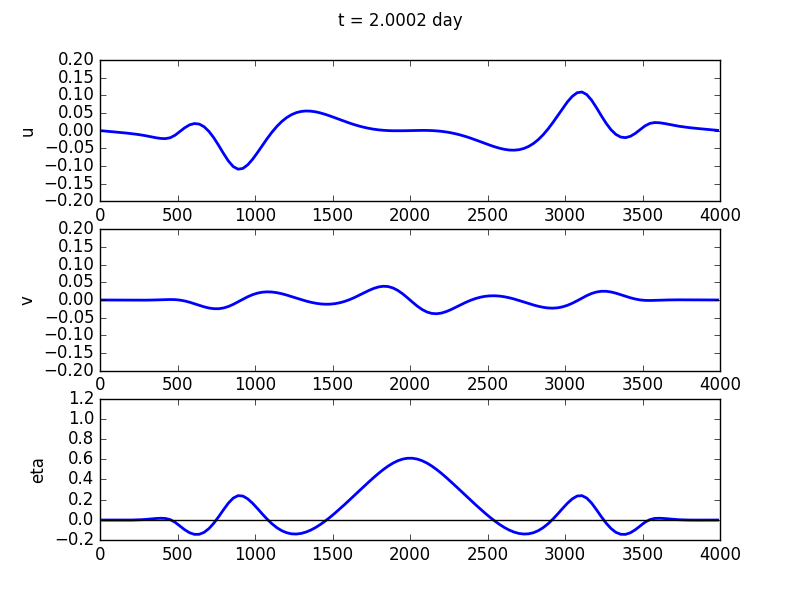
\includegraphics{ex1_fig1.png}
\caption{Final solution for the test case.}\end{figure}
\begin{figure}[htbp]
\centering
\capstart

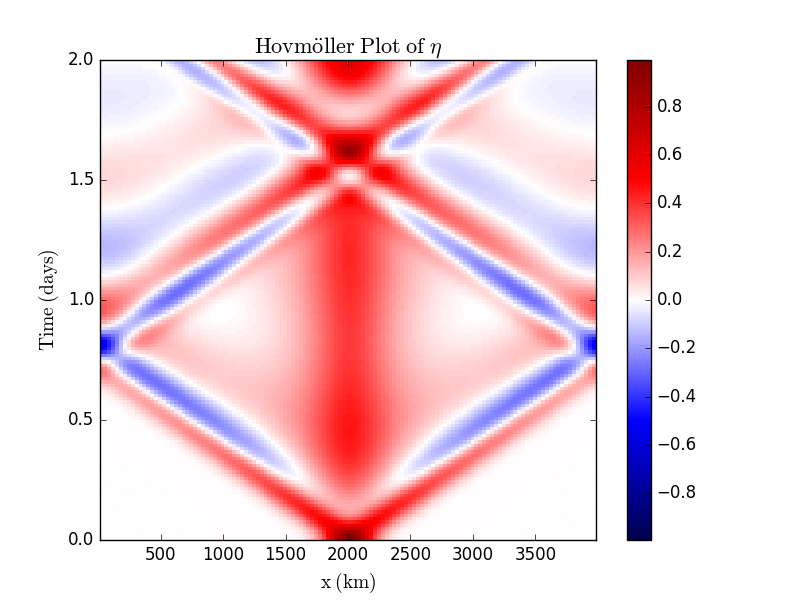
\includegraphics{ex1_fig2.png}
\caption{Hovmöller plot for the test case.}\end{figure}

<<<<<<< HEAD
There is a second example called example\_1D\_geoadjust2.py that begins
with a hyperbolic tangent profile instead if a Gaussian initial
condition.


\section{Geostrophic Adjustment: 2D and 1L}
\label{examples:geostrophic-adjustment-2d-and-1l}
The basic script is almost identical to the 1D case. The changes are as
follows:
=======
Note that to compute the derivatives in the case of a non-periodic
domain we impose either Dirichlet or Neumann boundary conditions. This
is done by doing odd and even extensions respectively. That is why in
1D, the simulation with walls does twice as much work as in the periodic
case. Similarly, if we have walls in 2D, that is doing four times as
much work.

At some point we should change walls to ’slip’ and allow for ’noslip’
boundary conditions as well.


\section{Geostrophic Adjustment: Two-Dimensions}
\label{examples:geostrophic-adjustment-two-dimensions}
The basic script is almost identical to the 1D case and can be found in
the examples folder with the title example\_2D\_geoadjust.py. The
changes are as follows:
>>>>>>> master
\begin{itemize}
\item {} 
Set \(Nx\) and \(Ny\) both equal to \(128\), and from
this we build a 2D grid.

\item {} 
<<<<<<< HEAD
Define the initial conditions on a 2D grid.

\item {} 
The plotting is different. We plot a 2D field using and we don’t do a
Hovmöller plot.

\end{itemize}


\section{Bickley Jet: 2D and 1L}
\label{examples:bickley-jet-2d-and-1l}
Following Poulin and Flierl (2003) and Irwin and Poulin (2014), we look
at the instability of a jet.


\chapter{Linear Stability Analysis}
\label{linear_stability::doc}\label{linear_stability:linear-stability-analysis}

\section{One-Layer Shallow Water}
\label{linear_stability:one-layer-shallow-water}
In this subsection we consider the one-layer reduced gravity RSW model
with topography below. We define the following:
\begin{itemize}
\item {} 
\(H\): mean depth of the layer

\item {} 
\(z=\eta\): height of the free surface

\item {} 
\(z=-H + \eta_B\): height of the topography.

\item {} 
\(h = H + \eta - \eta_B\): total depth of layer

\item {} 
\((u,v)\): horizontal velocity

\item {} 
\(g'\): reduced gravity

\item {} 
\(\rho_0\): reference density

\end{itemize}

The governing nonlinear equations are,
\begin{gather}
\begin{split}\begin{aligned}
\frac{\partial u}{\partial t} + {\vec u} \cdot \vec \nabla u - f v &
= - g \frac{\partial}{\partial x} \left( h + \eta_B \right) , \\
 \frac{\partial v}{\partial t} + {\vec u} \cdot \vec \nabla v + f u &
= - g \frac{\partial}{\partial y} \left( h + \eta_B \right) , \\
\frac{\partial h}{\partial t} + \vec\nabla \cdot \left( h \vec u_1 \right) & = 0.\end{aligned}\end{split}\notag
\end{gather}

\section{Basic State}
\label{linear_stability:basic-state}
To study shear flows in a meridional channel we consider solutions of
the form,
\begin{gather}
\begin{split}\begin{aligned}
u & = U_B(y), \\
v & = 0,\\
h & = H_B(y).\end{aligned}\end{split}\notag
\end{gather}
For this to be an exact solution we require that the flow is in
geostrophic balance,
\begin{gather}
\begin{split}f U_B = - g \frac{d}{dy}\left( H_B + \eta_B \right).\end{split}\notag
\end{gather}

\section{Perturbation}
\label{linear_stability:perturbation}
We perturb the basic state with infinitesimal quantities,
\begin{gather}
\begin{split}\begin{aligned}
u & = U_B(y) + u', \\
v & = 0     + v',\\
h & = H_B(y) + h'.\end{aligned}\end{split}\notag
\end{gather}
We substitute our perturbation into the governing equations and drop the
primes (for brevity) and cancelling out the geostrophic terms
\begin{gather}
\begin{split}\begin{aligned}
\frac{\partial u}{\partial t} + (u + U_B) \frac{\partial u}{\partial x} + v \frac{\partial}{\partial y} \left(u + U_B \right)  - f v & = - g \frac{\partial h}{\partial x}, \\
 \frac{\partial v}{\partial t}   + (u + U_B) \frac{\partial v}{\partial x} + v \frac{\partial v }{\partial y} + f u
 & = - g \frac{\partial h}{\partial y}, \\
\frac{\partial h}{\partial t}  + (u + U_B) \frac{\partial h}{\partial x}   + v \frac{\partial}{\partial y}(H_B + h)
+ (H_B + h)  & \left( \frac{\partial u}{\partial x} + \frac{\partial v}{\partial y} \right) =  0.\end{aligned}\end{split}\notag
\end{gather}
Now we neglect the quadratic terms to obtain the linearized equations,
\begin{gather}
\begin{split}\begin{aligned}
\frac{\partial u}{\partial t}
& = - U_B \frac{\partial u}{\partial x} + \left( f - \frac{d U_B}{d y}  \right) v  - g \frac{\partial h_1}{\partial x}, \\
 \frac{\partial v}{\partial t}    & =  - f u  - U_B \frac{\partial v}{\partial x}  - g \frac{\partial h_1}{\partial y}, \\
\frac{\partial h}{\partial t}   & = - H_B \frac{\partial u}{\partial x}    - v \frac{d H_B}{d y}
 - H_B \frac{\partial v}{\partial y} - U_B \frac{\partial h}{\partial x} .\end{aligned}\end{split}\notag
\end{gather}
Finally, we assume a normal mode decomposition in the zonal direction
and time,
\begin{gather}
\begin{split}\begin{aligned}
[u, v, h] = \mbox{Re}\left\{ e^{ik(x - c t)} [\hat u, ik \hat v, \hat h] \right\},\end{aligned}\end{split}\notag
\end{gather}
which we can substitute into the above equations to yield in the
inviscid limit
\begin{gather}
\begin{split}\begin{aligned}
c \hat u  &  = U_B \hat u - (f - \frac{dU_B}{dy}) \hat v + g \hat h, \\
c \hat v  &  =- \frac{f}{k^2} \hat u + U_B \hat v -\frac{ g}{k^2} \frac{d h}{d y}, \\
c \hat h  &=   H_B \hat u  +  \frac{d}{d y}\left(H_B \hat v\right) +  U_B \hat h.\end{aligned}\end{split}\notag
\end{gather}
=======
Specify the length of the domain in the zonal direction.

\item {} 
Define the initial conditions on a 2D grid.

\item {} 
The plotting is different. We plot a 2D field using pcolormesh and we
don’t do a Hovmöller plot.

\end{itemize}


\section{Bickley Jet: Two-Dimensions}
\label{examples:bickley-jet-two-dimensions}
Following Poulin and Flierl (2003) and Irwin and Poulin (2014), we look
at the instability of a Bickley jet. The script is called
example\_2D\_BickleyJet.py.

In this case we change the code to include the following lines.

\begin{Verbatim}[commandchars=\\\{\}]
\PYG{c}{\PYGZsh{} Define geometry}
\PYG{n}{sim}\PYG{o}{.}\PYG{n}{geomx}       \PYG{o}{=} \PYG{l+s}{\PYGZsq{}}\PYG{l+s}{periodic}\PYG{l+s}{\PYGZsq{}}
\PYG{n}{sim}\PYG{o}{.}\PYG{n}{geomy}       \PYG{o}{=} \PYG{l+s}{\PYGZsq{}}\PYG{l+s}{walls}\PYG{l+s}{\PYGZsq{}}

\PYG{c}{\PYGZsh{} Define grid and domain size}
\PYG{n}{sim}\PYG{o}{.}\PYG{n}{Lx}  \PYG{o}{=} \PYG{l+m+mf}{200e3}          \PYG{c}{\PYGZsh{} Domain extent               (m)}
\PYG{n}{sim}\PYG{o}{.}\PYG{n}{Ly}  \PYG{o}{=} \PYG{l+m+mf}{200e3}          \PYG{c}{\PYGZsh{} Domain extent               (m)}
\PYG{n}{sim}\PYG{o}{.}\PYG{n}{Nx}  \PYG{o}{=} \PYG{l+m+mi}{128}            \PYG{c}{\PYGZsh{} Grid points in x}
\PYG{n}{sim}\PYG{o}{.}\PYG{n}{Ny}  \PYG{o}{=} \PYG{l+m+mi}{128}            \PYG{c}{\PYGZsh{} Grid points in y}

\PYG{c}{\PYGZsh{} Bickley Jet initial conditions}
\PYG{c}{\PYGZsh{} First we define the jet}
\PYG{n}{Ljet} \PYG{o}{=} \PYG{l+m+mf}{20e3}            \PYG{c}{\PYGZsh{} Jet width}
\PYG{n}{amp}  \PYG{o}{=} \PYG{l+m+mf}{0.1}             \PYG{c}{\PYGZsh{} Elevation of free\PYGZhy{}surface in basic state}
\PYG{n}{sim}\PYG{o}{.}\PYG{n}{soln}\PYG{o}{.}\PYG{n}{h}\PYG{p}{[}\PYG{p}{:}\PYG{p}{,}\PYG{p}{:}\PYG{p}{,}\PYG{l+m+mi}{0}\PYG{p}{]} \PYG{o}{+}\PYG{o}{=} \PYG{o}{\PYGZhy{}}\PYG{n}{amp}\PYG{o}{*}\PYG{n}{np}\PYG{o}{.}\PYG{n}{tanh}\PYG{p}{(}\PYG{n}{sim}\PYG{o}{.}\PYG{n}{Y}\PYG{o}{/}\PYG{n}{Ljet}\PYG{p}{)}
\PYG{n}{sim}\PYG{o}{.}\PYG{n}{soln}\PYG{o}{.}\PYG{n}{u}\PYG{p}{[}\PYG{p}{:}\PYG{p}{,}\PYG{p}{:}\PYG{p}{,}\PYG{l+m+mi}{0}\PYG{p}{]}  \PYG{o}{=}  \PYG{n}{sim}\PYG{o}{.}\PYG{n}{g}\PYG{o}{*}\PYG{n}{amp}\PYG{o}{/}\PYG{p}{(}\PYG{n}{sim}\PYG{o}{.}\PYG{n}{f0}\PYG{o}{*}\PYG{n}{Ljet}\PYG{p}{)}\PYG{o}{/}\PYG{p}{(}\PYG{n}{np}\PYG{o}{.}\PYG{n}{cosh}\PYG{p}{(}\PYG{n}{sim}\PYG{o}{.}\PYG{n}{Y}\PYG{o}{/}\PYG{n}{Ljet}\PYG{p}{)}\PYG{o}{*}\PYG{o}{*}\PYG{l+m+mi}{2}\PYG{p}{)}
\PYG{c}{\PYGZsh{} Then we add on a random perturbation}
\PYG{n}{sim}\PYG{o}{.}\PYG{n}{soln}\PYG{o}{.}\PYG{n}{u}\PYG{p}{[}\PYG{p}{:}\PYG{p}{,}\PYG{p}{:}\PYG{p}{,}\PYG{l+m+mi}{0}\PYG{p}{]} \PYG{o}{+}\PYG{o}{=}  \PYG{l+m+mf}{2e\PYGZhy{}3}\PYG{o}{*}\PYG{n}{np}\PYG{o}{.}\PYG{n}{exp}\PYG{p}{(}\PYG{o}{\PYGZhy{}}\PYG{p}{(}\PYG{n}{sim}\PYG{o}{.}\PYG{n}{Y}\PYG{o}{/}\PYG{n}{Ljet}\PYG{p}{)}\PYG{o}{*}\PYG{o}{*}\PYG{l+m+mi}{2}\PYG{p}{)}\PYG{o}{*}\PYG{n}{np}\PYG{o}{.}\PYG{n}{random}\PYG{o}{.}\PYG{n}{randn}\PYG{p}{(}\PYG{n}{sim}\PYG{o}{.}\PYG{n}{Nx}\PYG{p}{,}\PYG{n}{sim}\PYG{o}{.}\PYG{n}{Ny}\PYG{p}{)}
\end{Verbatim}

>>>>>>> master

\chapter{Indices and tables}
\label{index:indices-and-tables}\begin{itemize}
\item {} 
\DUspan{xref,std,std-ref}{genindex}

\item {} 
\DUspan{xref,std,std-ref}{modindex}

\item {} 
\DUspan{xref,std,std-ref}{search}

\end{itemize}



\renewcommand{\indexname}{Index}
\printindex
\end{document}
